\section{项目事宜}

\noindent 本项目是基于图书的文本信息和图片信息来解决文本多分类任务。一般的AI项目流程可分为\textit{数据预处理、文本特征工程、建模和调参、评估以及部署构成}。通过本项目的实操,你将会体会到每个环节的细节如何去落地。



\subsection{项目的整个框架}

\noindent 整个项目框架如图~\ref{fig:project_mindmap}所示。下面对于图中每个模块做简要的描述,具体的细节请参考本文章后续的内容。

\begin{figure}[ht]
 \centering
 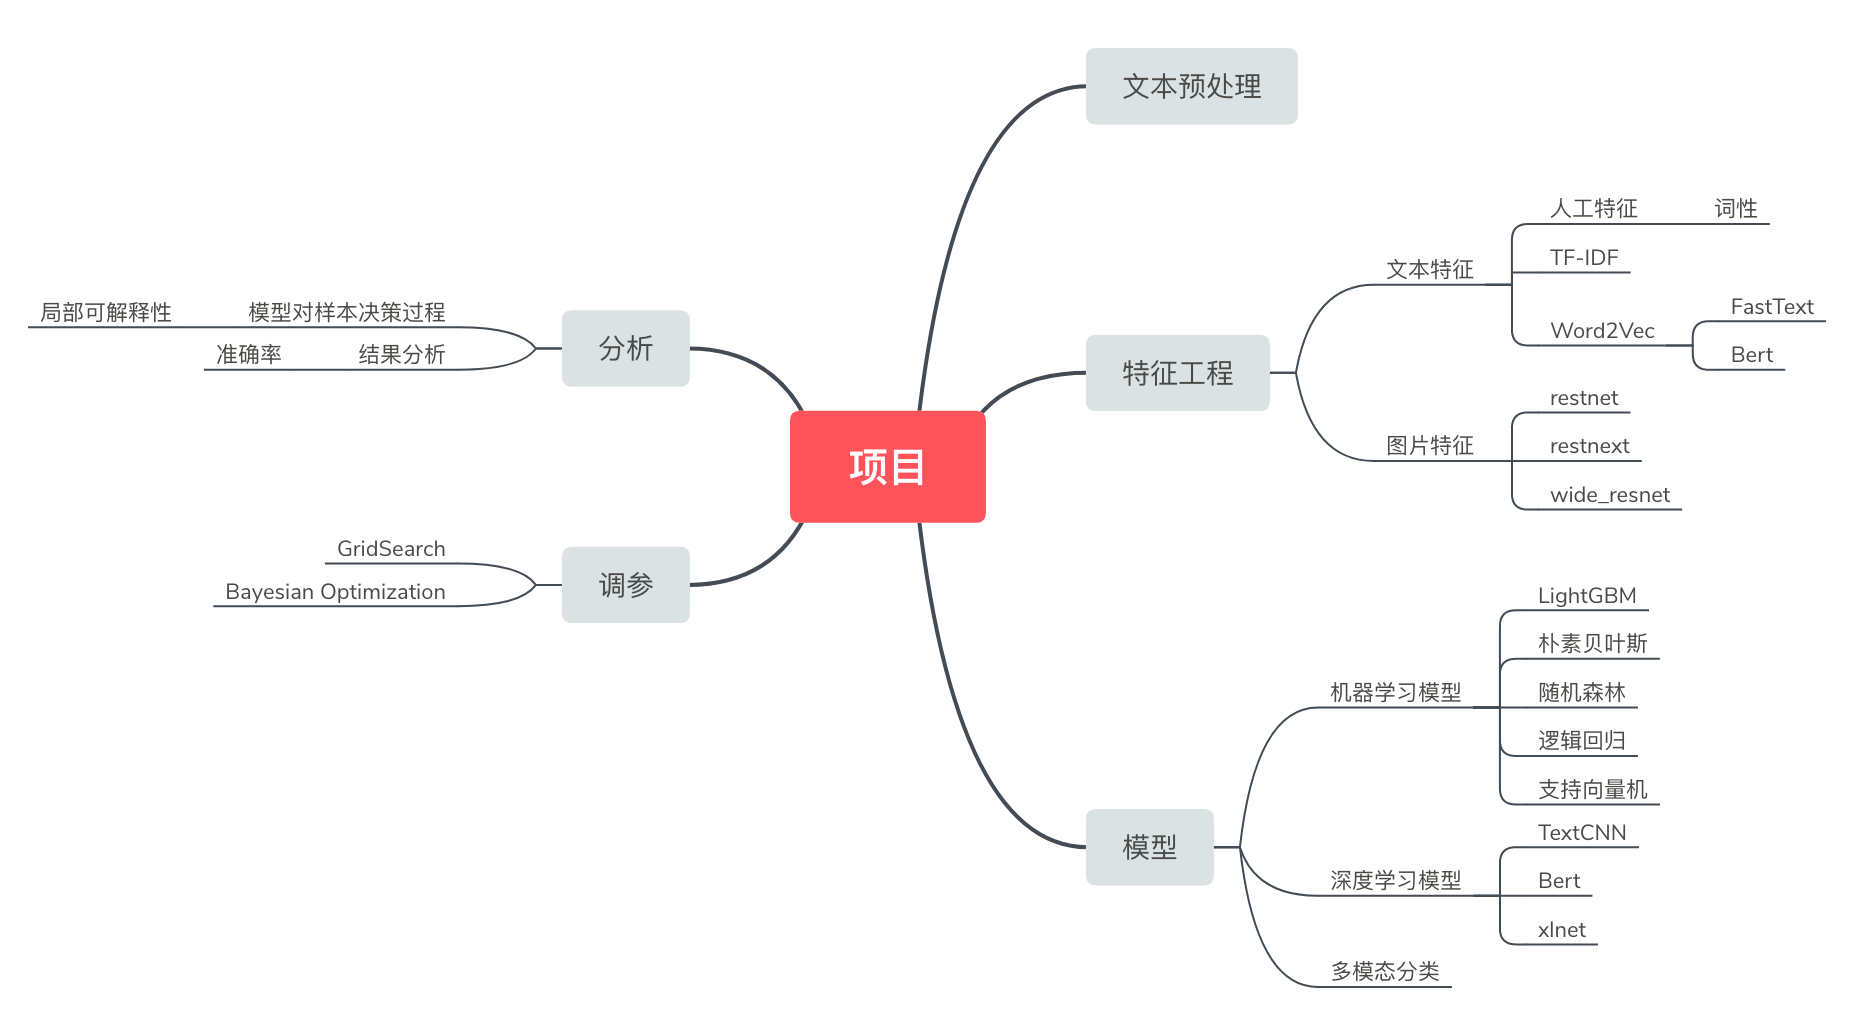
\includegraphics[height=7cm]{images/project_mindmap.jpg}
 \caption{京东图书分类项目模块架构图}
 \label{fig:project_mindmap}
\end{figure}

\begin{itemize}
    \item \textbf{特征工程}:这块涉及到文本和图片的特征。对于文本的特征,在本项目中需要使用\texttt{tf-idf~\cite{paik2013novel}}, 经典的预训练词向量(\texttt{FastText}, \texttt{BERT~\cite{DBLP:journals/corr/abs-1810-04805}})、以及人工抽取的一些特征如单词的词性、实体类别等。对于图片,我们将使用\texttt{ResNet~\cite{DBLP:journals/corr/HeZRS15}}等预训练模型来获得图片向量。等获取完文本和图片向量之后,我们会做特征的拼接来做多模态的训练。 
    \item \textbf{模型}:在训练过程中,你将有机会尝试使用各类经典的机器学习模型以及深度学习模型。很多模型已经提供给了大家,大部分模型不需要自己编写。  
    \item \textbf{调参}:对于模型的调参环节,我们选择使用\texttt{网格搜索}和\texttt{贝叶斯优化}搜索算法。后者相比前者可以缩小搜索空间,但同时也会增加每次的搜索代价,具体效率可以通过实验来体会。
    \item \textbf{分析}:评估模型的好坏通常都需要一个标准如准确率或者\texttt{F1-Score}。除此之外,目前对于深度学习模型来讲,很多时候都以黑盒子的形态来存在,我们很难判断为什么这个模型对于某些样本分类的很准确,对于某些样本分类错误。为了了解更多内部的机理,我们\textit{实现了基于词、短语以及词与词、短语与短语之间交互的可解释性模型},即针对一个样本,找出该样本中哪些词或者词组对模型分类的贡献度较大。
    \item \textbf{数据的不平衡处理}:另外,项目数据本身的类别不平衡:有些类别很多,有些类别则比较少,这对于训练模型来讲会有一定的挑战。项目中将使用\texttt{BalancedBaggingClassifier}、\texttt{SMOTE~\cite{DBLP:journals/corr/abs-1106-1813}} 和\texttt{ClusterCentroids}[3]等模型来解决上述问题。
\end{itemize}








